\documentclass[10pt,twocolumn,letterpaper]{article}

% \usepackage{cvpr}
\usepackage{times}
\usepackage{epsfig}
\usepackage{graphicx}
\usepackage{amsmath}
\usepackage{amssymb}

% Include other packages here, before hyperref.

% If you comment hyperref and then uncomment it, you should delete
% egpaper.aux before re-running latex.  (Or just hit 'q' on the first latex
% run, let it finish, and you should be clear).
\usepackage[pagebackref=true,breaklinks=true,letterpaper=true,colorlinks,bookmarks=false]{hyperref}

\begin{document}


%%%%%%%%% TITLE
\title{\LaTeX\ TITLE HERE }

\author{First Author\\
Institution1\\
Institution1 address\\
{\tt\small firstauthor@i1.org}
% For a paper whose authors are all at the same institution,
% omit the following lines up until the closing ``}''.
% Additional authors and addresses can be added with ``\and'',
% just like the second author.
% To save space, use either the email address or home page, not both
\and
Second Author\\
h
Institution2\\
First line of institution2 address\\
{\tt\small secondauthor@i2.org}
}

\maketitle
%\thispagestyle{empty}

%%%%%%%%% ABSTRACT
\begin{abstract}
Phenotyping at the plant level has crucial applications for highly valuable crops, species selection and botanical research. While two-dimensional imaging is sufficient for field-scale observation, individual monitoring requires three-dimensional imaging. It allows to reach a sufficient precision and level of information regarding the biological traits measured at this level. In this paper we present a 3D-scanning set-up that allows to reconstruct a plant in 3D organ-per-organ and produce a segmented point-cloud of the plant from 2D images taken at various viewpoints. Our method is fast and robust and requires little computational power as the complex step of segmentation is entirely processed at the image-level rather than the volume-level. The method we present relies on computer-vision neural network for the image segmentation. To bypass the problem of manual annotation required to train the network, we present a novel method which relies on 3D model of plants \emph{A. Thaliana} staged in a virtual environment to mimic the 3D scanner and acquire training images for the segmentation neural network. We present quantitative reconstruction results with the 3D virtual scanner and qualitative results with real \emph{A. Thaliana} plants. All the code is available on GitHub, and we address the issue of the ability to transfer the method to other plants by allowing a user to fine-tune the network on his own images. We show that the manual annotation of only two images is sufficient to obtain a reliable 3D reconstruction of a different plant, here a tomato plant.

\end{abstract}

%%%%%%%%% BODY TEXT
\section{Introduction}
% Plant architecture is a complex product where both genetic determinants and
% environmental factors interact in intricate developmental mechanisms during the
% plant’s life. Understanding this fascinating process is an active research field
% that requires precise measurements of plant structures at different scales.
% Scrutinizing plant architecture is also a cornerstone in agriculture, from
% breeding new varieties to daily monitoring in the field. In both cases,
% phenotyping must reconcile accuracy at the plant scale (from mm to meter range)
% with a high throughput. However, such phenotyping solutions are too expensive
% for most researchers or farmers. Their cost is due to the use of high-tech
% components or to their demanding development that requires competence in
% mechanics, robotics, sensors, computational analysis and database management. As
% a consequence, most phenotyping systems are huge platforms or machines achieving
% very high throughput to ensure a profitable investment.
%     Recently, the cost of many electronic devices dropped and support for open
% source hardware and software solutions is rising. Constant progress is made in
% computer vision to reconstruct precise 3D objects. However, state-of-the-art
% algorithms performs badly with plants: they lack robustness to variations in the
% conditions of acquisition and are not generic to handle all types of plants.
%     In this paper we are interested particularly in Phyllotaxy. This field
% studies the arrangement of botanical structures around axis of growth [1]. This
% is one of the most famous examples of regular patterns with mathematical
% properties in living organisms. While it is a dynamic interdisciplinary research
% front, there is no automated solution for phenotyping phyllotaxis yet.
%     In this context, we are prototyping an inexpensive, easy-to-build,
% easy-to-use robot for phenotyping plant architecture in 3D. It has a medium
% throughput that should fit the needs of small research teams or micro-farms.
% Despite the use of cheap and basic components, our challenge is to develop image
% analysis pipeline achieving high-precision in 3D phenotyping over a large
% diversity of plant architectures. As a first proof of concept, we tested an
% indoor set-up with the fine structure of the phyllotaxis of the model plant
% Arabidopsis thaliana.


% Large-scale phenotyping can help us understand biology but also to adapt
% cultures to a chang-
% ing environment. Working on well understood model plants like arabidopsis can
% both provide
% useful data to the biologists and is an important stepping stone to the study of
% more complex
% models: in-field imaging of crops, imaging of plant populations. . .
% Data collection and traits extractions are time-consuming process and a major
% bottleneck
% in plant phenotyping [13]. There is therefore a need of automated procedures to
% quickly
% c 2018. The copyright of this document resides with its authors.
% It may be distributed unchanged freely in print or electronic forms.2
% WINTZ, COLLIAUX, HANAPPE: EXTRACTION OF TRAITS FROM ARABIDOPSIS
% extract important parameters from live models. In this work, we propose a fully
% automated
% procedure to extract the structure of arabidopsis, including internode lengths
% and angles be-
% tween successive organs.

% Extracting plant fea-
% tures is a first step toward quantifying biomass and
% yield (Mathan et al., 2016), assessing flowering time and
% drought tolerance (Minervini et al., 2016), mapping
% genotypes to phenotypes (Balduzzi et al., 2017; Setter,
% 2012), and studying morphological properties of plant
% architectures (Conn et al., 2017a; Conn et al., 2017b;
% Bucksch et al., 2017; Li et al., 2018; Prusinkiewicz and
% Lindenmayer, 1996). Common phenotyping features of
% interest include the number, size, and shape of leaves (Wilf
% et al., 2016; Huang et al., 2018); plant height and growth
% rates (Madec et al., 2017); and branch lengths, diameters,
% and angles (Bucksch et al., 2017); among other


Plant architecture is a complex geometrical object. Due to both genetic and
environmental variations, organs evolve in patterns which present great diversity
both between species and among individuals of the same species. Automated
reconstruction of plant structure from lab or in-field acquisitions remains a challenge in computer
vision (ref). The most common method for complex measurements of plant structure
remains handmade measurements and is a major bottleneck in plant phenotyping
(ref).  The application of automated processing of plant structure are many: precise
quantifying of biomass and yield for agricultural crops, mapping genotypes to
phenotypes, estimating growth parameters of species, among other. (Find many
refs)

% Many different techniques can be used to non-invasively obtain plant data:
% point cloud from laser scans, color images from a single view point, depth
% cameras etc.

% In the last two years, deep convolutional networks have outperformed the state
% ofthe art in many visual recognition tasks, e.g. [7,3]. While convolutional
% networkshave  already  existed  for  a  long  time  [8],  their  success  was
% limited  due  to  thesize of the available training sets and the size of the
% considered networks. Thebreakthrough by Krizhevsky et al. [7] was due to
% supervised training of a largenetwork with 8 layers and millions of parameters
% on the ImageNet dataset with1 million training images. Since then, even larger
% and deeper networks have beentrained [12].
%

Since the founding of works of (ref. ), deep convolutional networks have shown
to be the state of the art method for many classification tasks. Several
networks (ref ref) leverage huge classification datasets (ImageNet) to provide pixel by
pixel semantic segmentation. They have been successfully used for plant organ
segmentation (ref ref ref), but are still limited to simple case with a very
small diversity in test datasets. Using simulated data to augment training
datasets is a method which have shown to improve neural network performance in
many fields (ref ref).

Plant architecture is a well studied research topic, and many generative model
of plant architecture have been developped in the last decades. Lindenmayer
systems are rewriting systems specifically developped to model plant growth.
They can be used to model arbitrary complex model of plants.

In this work, we propose to use plant models to train convolutional neural network for
identification of different plant organs. The specific target application of
our method is the identification of organs of the model plant Arabidopsis
thaliana. We describe a data augmentation model using plant models and HDRI
pictures to produce ground truth images, as well as a simple method for
fine-tuning on real word data. We then present qualitative results in various
acquisition condition to assert the robustness of our method.

\section{Related works}

The problem we address tackles 2D segmentation and 3D reconstruction of plants at individual level. The main fields of application  are experimental phenotyping in laboratories for phenomics and crop improvement \cite{tisne_phenoscope:_2013,perez-sanz_plant_2017}, as well as in-field monitoring of highly valuable crops \cite{hoffmann_fluorescence_2015, fiorani_future_2013}. The common approach in phenotyping is through 2D-imaging for it is fast, accessible and non-invasive. It allows to retrieve health-status, stress response and growth information through RGB, fluorescence and spectral images \cite{li_review_2014}. However due to the highly complex architecture of the plants, 3D information is necessary to monitor more specific traits like organ volume, phyllotaxis. \\
There are several possible methods to reconstruct a plant in 3D. First set of possibility is active reconstruction with lasers. LIDARs (Light Detection and Ranging) have been used to reconstruct plants in 3D to monitor growth and height \cite{garrido_3d_2015}. This method is sensitive to noise and time consuming as it has to scan the whole object point by point. It is also very sensitive to movement since its measure depends on travel length. A variation of LIDAR is laser light section scanner which projects a line on the plant instead of a point, allowing a faster reconstruction. It can be used to monitor plant spacing for example \cite{shi_automatic_2013}. \\
Another method is to project structured light on the plant. The deformation of the structure on the plants allows to compute the 3D depth of the scene. A sensor often used for this technique on plants is Kinect \cite{paulus_low-cost_2014, nguyen_structured_2015}, but it is poorly resolved and sensitive to sunlight.\\
3D reconstruction can also be achieved from multi-view 2D images. One method, Structure-from-motion, is to identify key-points from an image to another to reconstruct the plant in 3D such as corn in a field \cite{sodhi_-field_2017}. Another 2D-based method, space carving, method \cite{kutulakos_theory_1999} has already been used to reconstruct plants in 3D \cite{schonberger_structure--motion_2016} and it is the one we explored.\\
In the previously cited methods when a paper suggests a segmentation method, it is usually directly on the 3D data and not on the RGB images \cite{santos_automatic_nodate-1}. Yet a few papers report the use of 2D-image segmentation as the basis of the 3D segmentation. From different points of view it is possible to acquire a 3D representation of the plant, and by segmenting the images, it is possible to acquire a 3D segmented representation of the plant. The 2D pixel-wise image segmentation is achieved with machine learning and computer vision neural-networks. This approach has been suggested by \cite{kalogerakis_3d_2017} on the dataset ShapeNetCore, and an inspired approach has been presented in the context of plant phenotyping \cite{shi_plant-part_2019}. As an improvement we present an approach relying in more recent and efficient 2D segmentation neural network and exploiting an artificially-generated plant dataset of images which allows to by-pass the challenge of manual data-annotation.\\
 Simulated rendering of plants for semantic segmentation have already been developed, e.g.~\cite{duboudin_toward_2019, ward_deep_2018} but to the authors' knowledge they don't account for plant 3D geometry in the learning process. This limits applications to simple identification of scene objects relying on texture and basic shape only.



\section{Material and Methods}
\paragraph{Target applicative setup.}
To acquire plant images in a real world application scenario, we use a home made solution as a 3D
scanner. It consists in a X-Carve~\cite{xcarve} CNC Cartesian arm, combined with a
custom-made pan-tilt camera mount. This setup therefore has five degrees of freedom.
A Sony RX0 \alien{RGB }{}camera \alien{with $1920 \times 1060$ resolution}{} is mounted on the camera mount and is controlled using a Wifi interface. This allows for views from any point in space in a box containing
the imaged plant. The set-up in presented in \cite{wintz_automated_nodate}.

\paragraph{Virtual plants.}

The \tim{generative plant models}{virtual plants} were designed with
OpenAlea~\cite{pradal2009plantgl}. OpenAlea is an open source software
suite developped by INRIA to provide tools for plant architecture
modelling. \tim{The model plant \emph{Arabidopsis Thaliana} was chosen to
illustrate the methods in the paper, because it is a well-studied
plant and is a subject of active interest for many biologists.}{}

\tim{A generative model of \emph{A. Thaliana} was specifically
written in the L-py programming language. L-py is a python extension,
part of OpenAlea, which implements L-systems.}{3D meshes of \emph{A.
Thaliana} were designed with the L-Py library from OpenAlea, which
is a python implementation of L-system.} L-systems were developped
in 1968 by Aristid Lindenmayer~\cite{prusinkiewicz2012algorithmic}
to model plant growth.  It is a generative grammar that allows to
grow a virtual plant using symbols, shapes and constraints derived
\tim{from}{for} plant growth observation.

Formally it is called a rewriting system, or formal grammar. It
comprises:

\begin{itemize}
    \item A vocabulary V containing the \emph{modules} of the
    system. For plant generation it will represent an architectural
    element of the plant (apex, internode, leaf) and associated
    parameters (age, length, etc) \item An initial \emph{axiom}
    or state $s_0$ corresponding to the virtual plant at $t_0$. It
    is a string of elements from the vocabulary.  \item A set
    of \emph{production} rules to iterate in order to model
    the growth. They will be applied in parallel to each variable
    element from the string of the previous state. They are composed
    of a \emph{predecessor}, to identify the elements that will be
    replaced by a \emph{successor}.
\end{itemize}

\tim{Randomness can be added to the models by assigining different
probabilities to the set for rules. This allow to produce different
looking individual plants from a single set of rules. \alien{}{Our L-py model
for \emph{A. Thaliana} can be found online \cite{Lpy_godin}.}}{}

The strings can then be represented graphically in 3D using OpenAlea's
PlantGL (Figure\ref{fig:lpy}). Figure~\ref{fig:lpy} illustrates a virtual specimen
of A. Thaliana obtained using the lpy generative model at different timesteps.

The A. Thaliana models comprised 5 different types of organs: fruit, stem, pedicel, leaf and flower.

\begin{figure}[h!]
    \centering 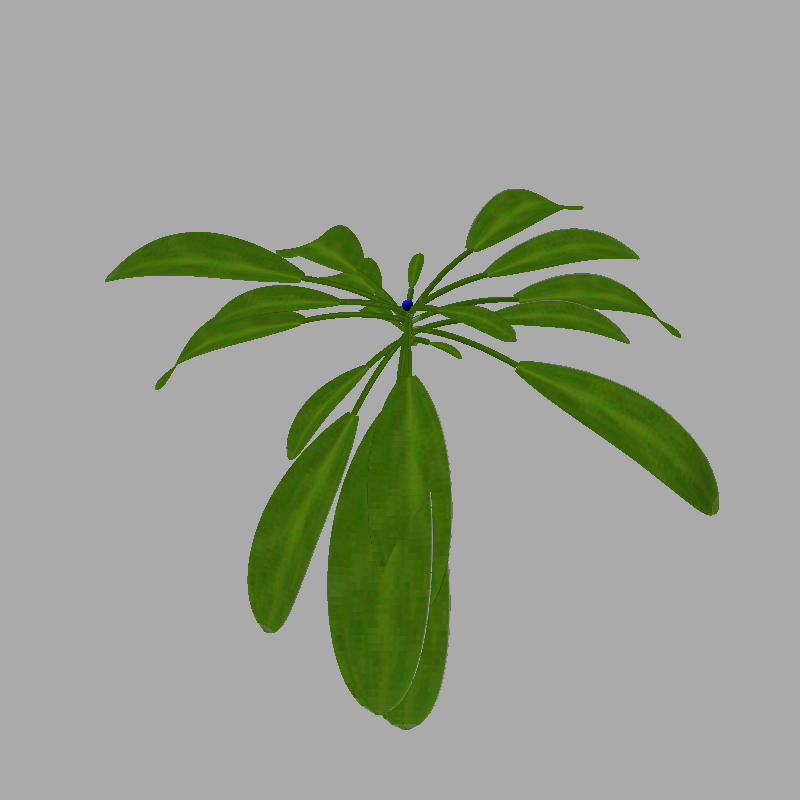
\includegraphics[width = 0.3\linewidth]{figures/10d.png}\hspace{1em}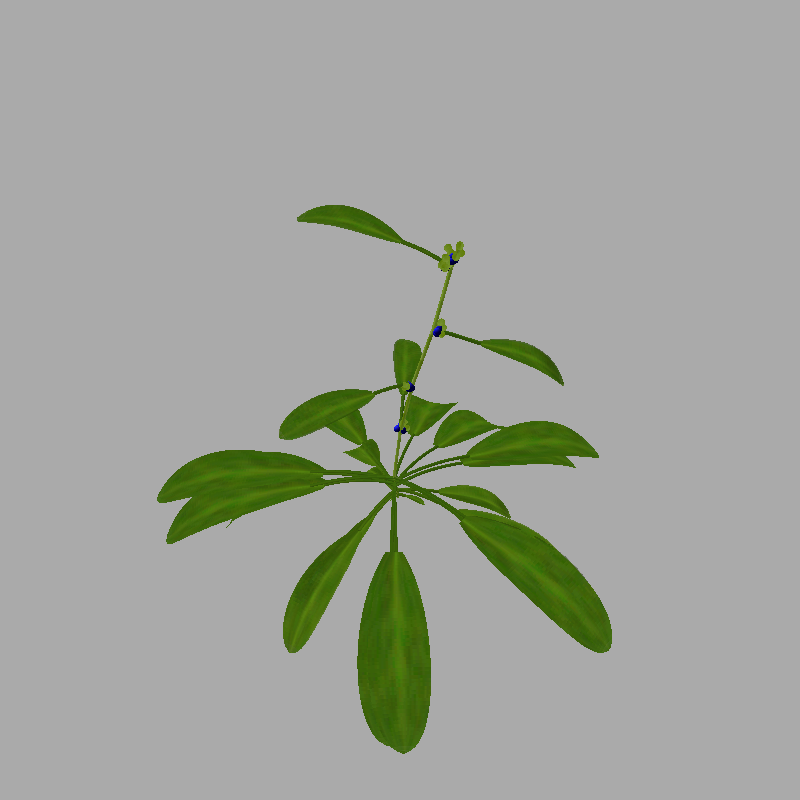
\includegraphics[width = 0.3\linewidth]{figures/20d.png}

    \vspace{0.9em}
    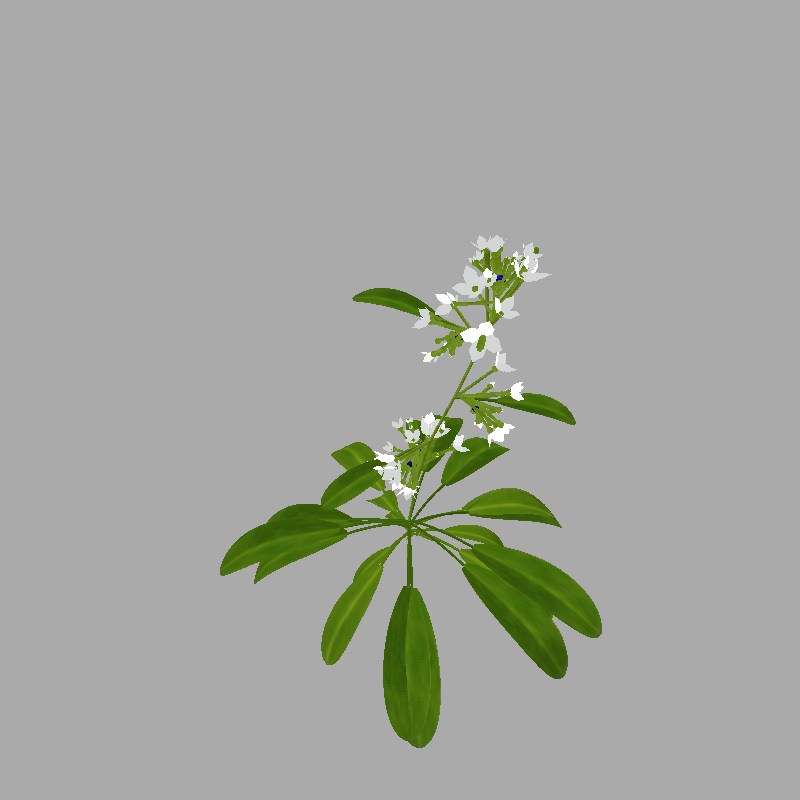
\includegraphics[width = 0.3\linewidth]{figures/30d.png}\hspace{1em}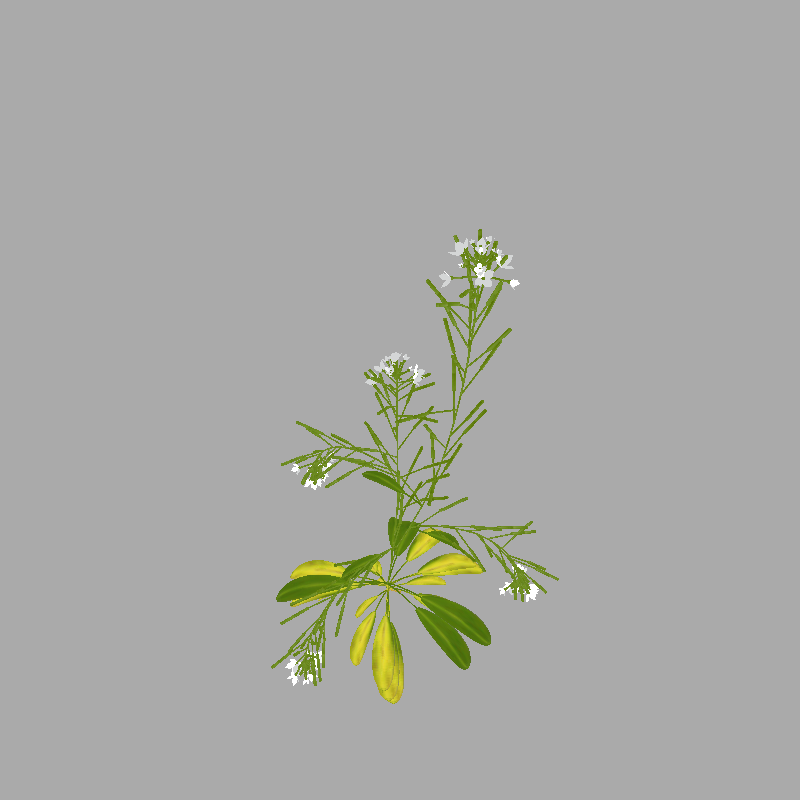
\includegraphics[width = 0.3\linewidth]{figures/40d.png}
    \caption{An example of simulated \emph{Arabidopsis thaliana} using L-py. The four figures are representation of the same
    simulation after 240 (top left), 480 (top right), 720 (bottom left) and 960 (bottom right) iterations of the
    L-system.} \label{fig:lpy}
\end{figure}


\tim{The generated plant models are exported as meshes using the
standard OBJ format.}{}

\paragraph{Virtual scanner.} \tim{The open source software
Blender~\cite{blender} was chosen for the rendering part. The blender
Eevee renderer allows for fast and realistic looking rendering of
scenes and the python bpy modules allows for easy scripting.}{}

\tim{The idea is to provide a simulated environment similar to
the real application described above.}{} \tim{A python script using bpy and
flask}{An API} was \tim{written}{implemented} to
generate and visualise the generated plant 3D models in Blender.
\tim{HTTP requests allow us to easily load different plant models and
backgrounds into the Blender scene, to move the loaded object,
as well as change the camera position, rotation and its intrinsic
parameters. The rendering of the scene into an image can also
be triggered by a simple request. This enables us to take pictures of the
model around the plant, as we would on the real world setup~(Figure
\ref{fig:plants}).}{The 3D models are loaded in a virtual environment
and virtual cameras are used to take pictures of the
model~(Figure \ref{fig:plants}).}

To further increase the diversity of the simulated dataset and prevent
overfitting on the chosen plant textures, random colors are taken
from a reference image and applied as the base color of the plant material.

\tim{The scene background }{The plant is placed in a virtual background. It} is a $360^{\circ}$
\tim{real world picture}{image} and rendering it in blender reproduces the
original scene lighting\tim{. In order to increase the complexity of the
images acquired with the virtual scanner, s}{S}everal sets of backgrounds were
used, without limitations on the lighting environement -- night, daylight,
sunset -- or the type of scene -- indoor or outdoor. A simulated flash light is
triggered with a random level of intensity to simulate different artifical lighting condition during the
acquisition of real life pictures.

\begin{figure}[h]
    \centering 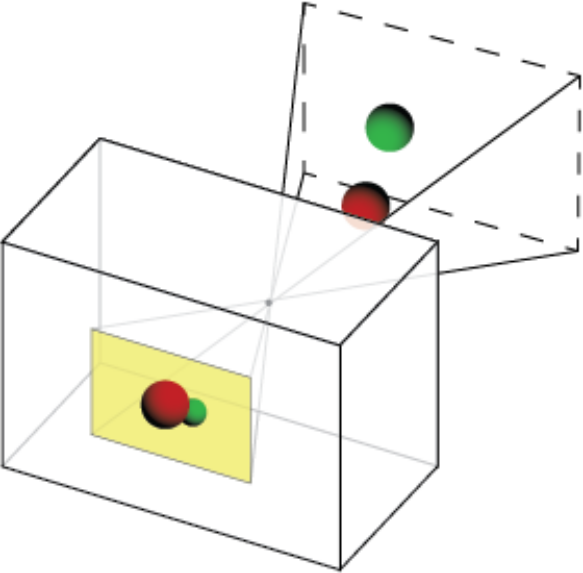
\includegraphics[width=0.3\linewidth]{figures/pinhole.png}
    \caption{Illustration of 2D overlapping due to perspective
    projection } \label{fig:pinhole}
\end{figure}

The \tim{ground truth plant part segmentation is}{virtual labels are} acquired by rendering the plant material by material, with one material per
\tim{plant part}{organ}~(Figure \ref{fig:plants}). The
\tim{plant parts}{organs} considered for \emph{A. Thaliana} are leaf, stem, flower,
fruit and peduncle. \tim{As we will see later for the 3D reconstruction, i}{I}n the pinhole model \cite{sturm_pinhole_2014} we use for 3D to 2D
projection, a whole line in 3D projects onto a single pixel (Figure
\ref{fig:pinhole}). As a consequence, a single pixel can belong to
several classes depending on the organs crossed by the line. The
labelling method takes this plurality into account by generating a
ground truth image for each class.

\begin{figure}[h]
    \centering 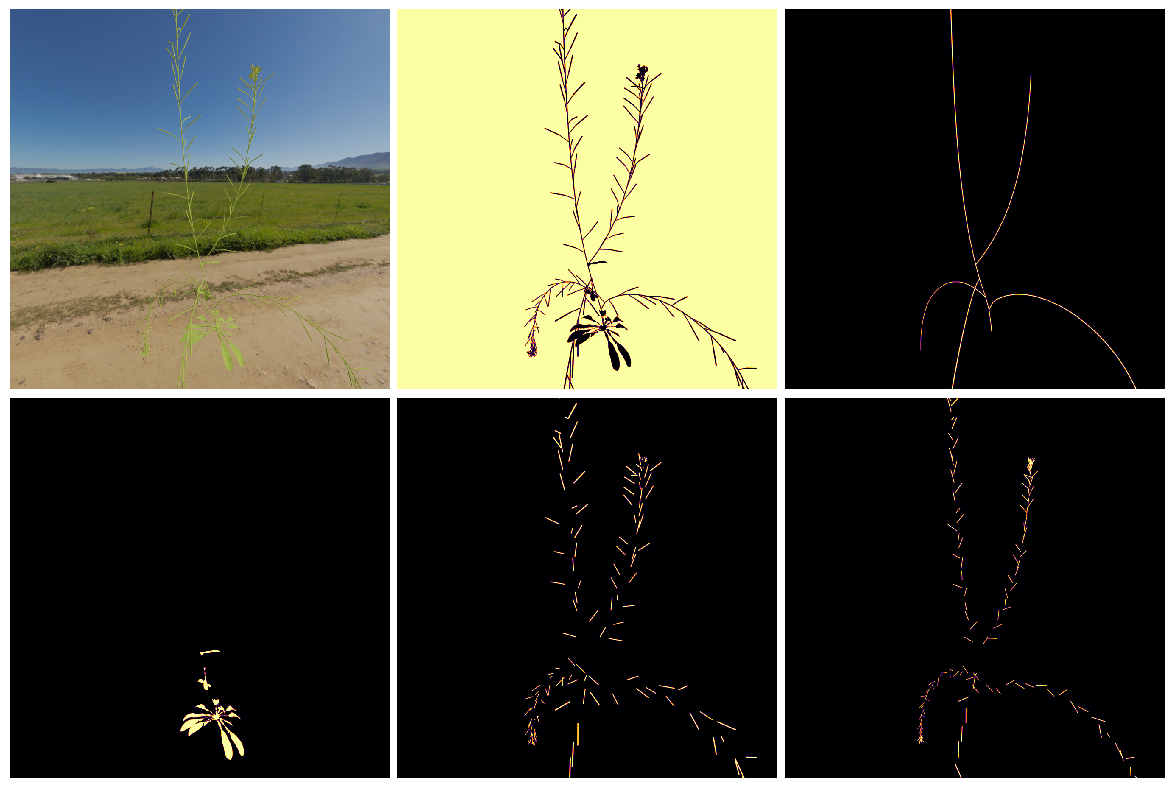
\includegraphics[width = 0.9\linewidth]{figures/Images_and_labels.png}
    \caption{Example of virtual training images and all labels}
    \label{fig:plants}
\end{figure}

\tim{The virtual scanner was used to generate a training dataset of plant
images with plant part segmentation 
for the training of neural networks.}{}


% \paragraph{3D ground truth.} The 3D virtual plants were
% used to train and evaluate the 3D reconstruction. The
% virtual mesh is regularly subsampled with CloudCompare
% \cite{girardeau-montaut_cloudcompare-open_2011} in order to get
% a density matching the voxel density in the volume to carve (see
% space carving section for explanations). Then this 3D point cloud is
% voxellized and each voxel of the volume to carve acquires an organ
% class, or class 0 (background) if it is not part of the plant. Then
% the vector is saved in a sparse representation to save memory. For the
% trainings, the data generator reads the sparse vector and encodes it
% in a dense representation to compare it to the predicted classes. It
% is needed to densify it because PyTorch can't backpropagate easily
% through a sparse representation.

%To train the classification on real plants, it was first considered
% to print a known plant model in 3D with Sculpteo, however the stem of
% the model wasn't thick enough and it buckled during the printing. We
% also considered to use an opensource dataset, however most segmented 3D
% dataset aimed for reconstruction are provided in Lidar or RGB-D data,
% and not from RGB to 3D. Therefore we decided to restrict ourselves to
% 3D virtual plants. We also used the 3D reconstructed models with the
% initial space-carving approach implemented previously in the pipeline
% \cite{wintz_automated_nodate} for comparison.


\paragraph{Image segmentation.} The objective of image \tim{semantic}{} segmentation is
to convert an input image in a stack of probability maps of the same
dimension as the image. \tim{If $C$ is the number of different classes,
semantic segmentation produces $C$ output images with values between $0$ and $1$,
giving for each pixel of the input image the probability of that pixel
belonging to the corresponding class.}{For C classes there will be C probability
maps, each corresponding to one class. The value of a pixel in the
probability map of class k is the probability that this pixel belongs
to the organ-type k in the original image.}


\tim{To produce such semantic probability maps, we used a segmentation
convolutional neural network~\cite{guo_review_2018}}{The image segmentation was performed using segmentation convolutional
neural network \cite{guo_review_2018}}. \tim{These}{Such} segmentation networks
are based on a contracting structure from an image to a low dimension\tim{al}{}
feature space, \tim{called the \emph{latent space}}{}, which encodes the content of the image. It is branched
to a symmetric expanding structure that translates the information from
the feature space to an image similar to the original one, but with
only the content of interest reconstructed. The contracting structure
is directly inspired from classification neural networks, and made
of convolution layers, non-linearities and down-pooling layers. The
convolution kernels allow to filter the information to emphasize
the content, and the down-pooling allows to reduce the dimension
of the information. The expanding structure reproduces the path in
the other direction, with up-pooling layers and convolutions. The
spatial information is re-injected to reconstruct the image properly,
by providing the down-pooling coordinates from the contracting phase.

\begin{figure}[h!]
    \centering 
\includegraphics[scale = 0.25]{figures/blank.png}
    \caption{Example of segmentation network: the U-Net architecture
    \cite{ronneberger_u-net:_2015}} \label{fig:unet}
\end{figure}

\tim{We decided to use a neural network architecture inspired by}{The structure tested was inspired from}
U-Net~\cite{ronneberger_u-net:_2015}. However, \tim{to leverage the power of
already existing labeled datasets}{}, the contracting
structure, or encoder, was replaced by a classification network trained
on ImageNet, and with six classes to segment. \tim{Thanks to the great diversity
in the ImageNet dataset, t}{T}his classification
structure has already \tim{learned}{been trained} to encode the semantic
representation of an image in the latent space. \tim{The classification network that we used is}{We tested}
ResNet~\cite{he_deep_2015} which is a deep neural network where inputs
from previous layers are regularly reinjected into deeper layers
in order to maintain the geometry and avoid vanishing gradients
\cite{hochreiter_vanishing_1998}.

\paragraph{Deep learning training} The network was trained with
images from the virtual scanner. \alien{The training set consisted of 2520 images (896x896 pixels), 18 views of 140 different virtual models. The distance and position of the camera around the plant varied to offer more diversity.}{TODO(Describe the path, dimension of the images). The dataset comprised TODO(Number of images)} To make the network robust to images and lighting conditions that are not in the dataset, we artificially augment the dataset by adding \alien{gaussian noise ($\sigma$ = 0.01) and random rotations (Figure \ref{fig:trainset}). The images were normalized to correspond to the mean and variance of the training set of ImageNet, on which was initially trained the semantic structure (mean: $(0.485, 0.456, 0.406)$ standard-deviation: $(0.229, 0.224, 0.225)$)}{TODO(add gaussian noise, change contrast, rotation, déformation, more?).}. 
The dataset was split into 3 sets:

\begin{itemize}
    \item a training set to train the network (70\% of the dataset)
    \item a validation set on which the network is not trained and
    is used to evaluate and compare the different networks (7\%
    of the dataset) \item a test set used at the very end on the
    selected architecture (23\% of the dataset)
\end{itemize}

\begin{figure}[h!]
	\centering 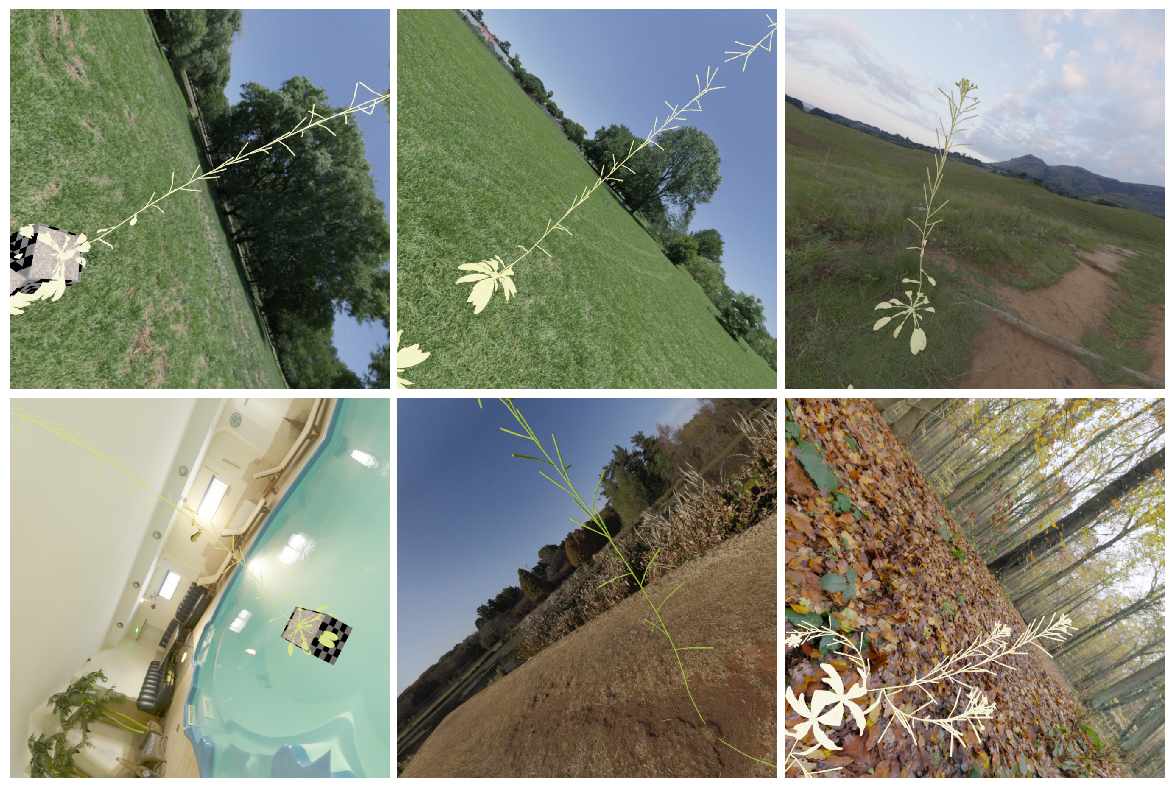
\includegraphics[width = 0.9\linewidth]{figures/vscan_sample.png}
	\caption{Sample of the training set (before normalization)} \label{fig:trainset}
\end{figure}


To evaluate the segmentation of the images, a combination of
metrics were used. As it is a multiclass problem, a sigmoid is
applied to each output in order to contain the numerical range of
the predictions. First crossentropy was used, it is a per-pixel
metric. It represents the uncertainty of the prediction compared to
the ground-truth. If the class of a pixel has a very low predicted
probability, it will highly penalise the loss. If the probability
is close to one, the contribution to the loss is close to zero. The
notion of entropy represents this discrepancy between the ground truth
distribution and the predicted distribution. It is naturally translated
at the mathematical level with the negative of the logarithm.

\begin{equation}
    L =-\sum_i^n\sum_k^C{y^k_{i, gt}\ln(y_{\textrm{i},
    \textrm{pred}}^k)}
\end{equation}

Where n is the number of pixels in the image, C the number of possible
classes, $y_{gt}^k = 1$ if pixel i is in class k, 0 otherwise, and
$y_ {\textrm{i}, \textrm{pred}}^k = p(\textrm{label}(y_{\textrm{i},
\textrm{gt}}) = k)$.

The second loss we used was the Dice coefficient, which theoretically
writes as:

\begin{equation}
    s = 1 - \frac{1}{n}\sum_{i=1}^n\sum_{k=0}^{C}y_{\textrm{i},
    \textrm{gt}} y_{\textrm{i}, \textrm{pred}}^k
\end{equation}


This coefficient compares the number of right predictions to the
number of samples, for each class. In practice, the product of the
ground truth by the predictions is summed, so that only the prediction
of the right class contributes to the sum. For example for point n,
the class is k, and the prediction for class k is $p_k$, the loss
for point n will be $1 - \frac{2p_k}{2} = 1 - p_k$. The total loss
is computed vector-wise, and lies between 0 and 1.


We used the mean of these two losses for the training, as the
crossentropy has more stable gradients, but the Dice loss is what we
want to minimise, and is less sensitive to class imbalance.


\paragraph{Fine-tuning.} Our network was trained on virtual \emph{A.
Thaliana} model but aims at reconstructing real plants. \alien{Although the training performs well for real \emph{A. Thaliana}, it transfers poorly to other species with large anatomical differences. }{Therefore when
the virtual plants fail at reproducing the complexity of real plants,
the network can perform poorly. The network also fails when confronted
to other plant species with very different traits.} Therefore we
conceived a simple interface that allows the user to manually label a
few images of interest (two or three images is enough), then run the training
of the network on this small dataset. This way, the network will be
able to segment similar images with correct classes.
\alien{The interface uses LabelMe \cite{russell_labelme:_2008} for manual annotations, and runs the training on these images for 20 epochs. This generates a segmentation network specialized for the new species, starting from the network trained on the virtual plant models of \emph{A. Thaliana}.}{}


% \paragraph{Space Carving.} We used space-carving to reconstructi
% the palnts in 3D from the 2D images. The space carving
% \cite{kutulakos_theory_1999} is a photogrammetric approach which uses
% pictures of an object from different point of views to reconstruct
% an object in 3D. To simplify the explanation we will take the example
% of the original space carving paper \cite{kutulakos_theory_1999}. Let
% the objective be to reconstruct a sculpture in 3D. The cameras circle
% a volume of interest that contains the cube and take $N$ pictures
% at regular intervals. Each picture will be pre-processed, with a
% masking step: on each image the mask will give the probability that
% the pixel belongs or not to the sculpture. Then, the surrounded volume
% is computed virtually, and each voxel of the volume is projected onto
% each masked view. If a voxel has projected onto the sculpture for each
% 2D-view, it is part of the 3D-sculpture. Otherwise it is part of the
% background: voxel after voxel, the volume is carved into the shape of
% the object. The main limitation of this technique is that the problem
% is ill-posed and the reconstructed object will be a \emph{photo
% hull} \cite{kutulakos_theory_1999} of the desired object, that is an
% object which is the union of all objects derivable from the multi-view
% observation. It can cause problems for highly curved or hollow objects,
% but in the case of plants it is not a major limitation.

\paragraph{Backprojection. } To reconstruct the 3D model from segmented 2D
pictures, we use a backprojection algorithm. It is an algorithm similar to 
the classical space carving algorithm~\cite{kutulakos_theory_1999}, which computes a 3D visual hull from
projections of binary masks of an object on 2D views.

Camera poses and intrinsic
parameters are either estimated using a structure from motion algorithm -- in
this work, we used the open source software Colmap~\cite{schoenberger2016mvs,
schoenberger2016sfm} -- or, in the case of simulated images, they are provided
as ground truth image metadata. If $N$ is the number of views taken for a given plant
scan, we thus have projection models $\pi_i,i \in \{1,\cdots, N\}$,
such that for any point $x \in \mathbb{R}^3$ of the world, $\pi_i ({x})$ is the
pixel coordinate of point ${x}$ in view $i$. Let $\Omega = [0,w]
\times [0,h]$ be the pixel domain for each image, and

$$
I(x) = \{ i \in
\{1,\cdots, N \} : \pi_i(x) \in \Omega \}
$$
be the set of views for which point
$x$ projects inside the pixel domain of the corresponding image. Then, for each
class $k \in \{ 1,\cdots, C \}$, the score $p_k(x)$ of class $k$ is given as:

$$
\log p_k(x) = \sum_{i\in I(x)} \log ( p_{i,k} (\pi_i(x) ),
$$
where $p_{i,k} (y)$ is the output of the segmentation network in the $i$th view
at pixel $y$.

Intuitively, it gives the log probability of any given class, assuming that the
probabilities for each of the classes projected on the images are independent
random variables.

The space is discretized into a fixed size voxel grid, and $p_k$ is computed at every
point of the grid. Then, the corresponding voxel is attributed the class which
yields the highest score. To convert the voxel grid into a labeled point cloud,
we use a level set algorithm~\ref{algorithm:pcdn}. The signed distance function is computed using a
fast marching algorithm in scipy~\ref{scipy}.

\begin{algorithm}
    \caption{From voxel grid to point cloud}
    \label{algorithm:pcdn}
    \begin{algorithmic}[1]
        \Function{PointCloud}{V}
        \State $D \gets \Call{SignedDistance}{V == 1}$
        \State $\nabla D \gets \Call{Gradient}{D}$
        \State $points \gets []$
        \State $normals \gets []$
        \For{$v \in V : |D[v]| < \sqrt{2} / 2$ }

        \Comment{Loop on all boundary points.}
            \State $n \gets \nabla D [v] / \Vert \nabla D [v] \Vert$
            \State $v_1 \gets v + D[v] * n$
            \State $\Call{Append}{points, v_1}$
            \State $\Call{Append}{normals, n}$
        \EndFor{}
        \State \textbf{return} $points, normals$
        \EndFunction
    \end{algorithmic}
\end{algorithm}


\section{Results and Discussions}
\paragraph{Testing methods.} The test data is composed of four
distinct datasets:
\begin{enumerate}[A.]
    \item A simulated dataset similar to the training dataset (14 different individuals, 1008 images)
    \item A small annotated set of plants from real Arabidopsis thaliana (4 different individuals, 6 images);
    \item A larger set of real Arabidopsis thaliana for qualitative evaluation (12 different indivudals, 864 images);
    \item A set of real images from another plant (tomato) to evaluate the possibility of transfering the learning onto other species of plants (TODO).
\end{enumerate}
All datasets will be available there: TODO.

Evaluation is done both on the 2D segmentation and on the resulting segmented 3D point cloud. For datasets A and B,
we present a class by class quantitative evaluation of the 2D segmentation method. For dataset A, we additionally  provide
class by class quantitative evaluation of the 3D voxel segmentation, as well as a comparison of output point clouds
to the ground truth given by L-Py. For dataset C, we provide qualitative assessment of the results of the segmentation,
both in 2D and in 3D. For dataset D, we restrict ourselves to qualitative evaluation of the 2D segmentation.

The background class is not considered as a class in itself in the evaluation, but is presented in the qualitative example. It
is only used for contrast when reconstructing point cloud from voxel data.

\paragraph{2D Segmentation and 3D Segmentation on dataset A.}
Images from datasets A are segmented used the trained neural network. Then, the results of 2D segmentation are
compared to the ground truth provided by the blender simulation. Figure~\ref{fig:seg2d_res} presents a sample from
dataset A and its segmentation.

\begin{figure}
    \centering 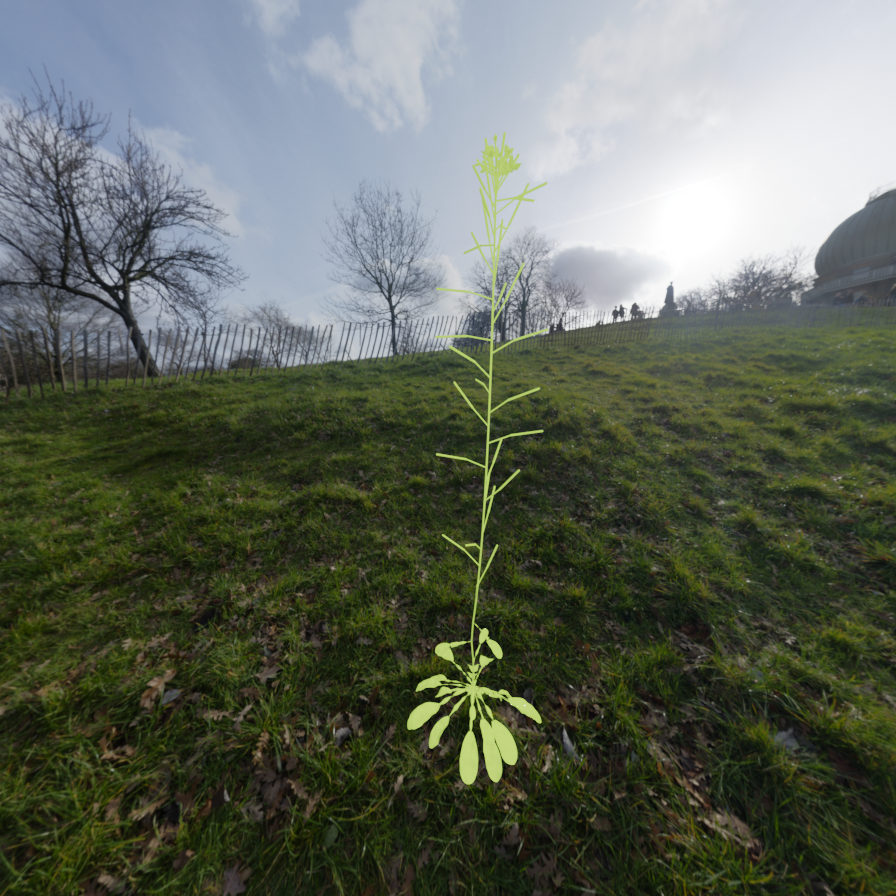
\includegraphics[width = 0.25\linewidth]{figures/00000_rgb.png}\quad
    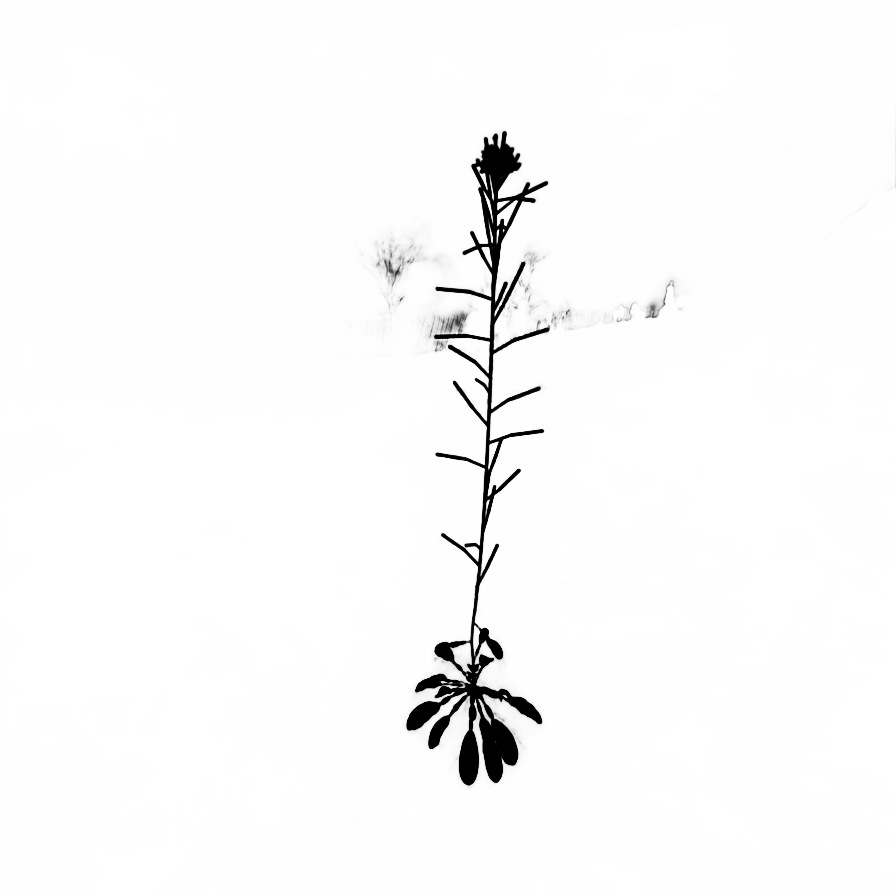
\includegraphics[width = 0.25\linewidth]{figures/000_background.png}\quad
    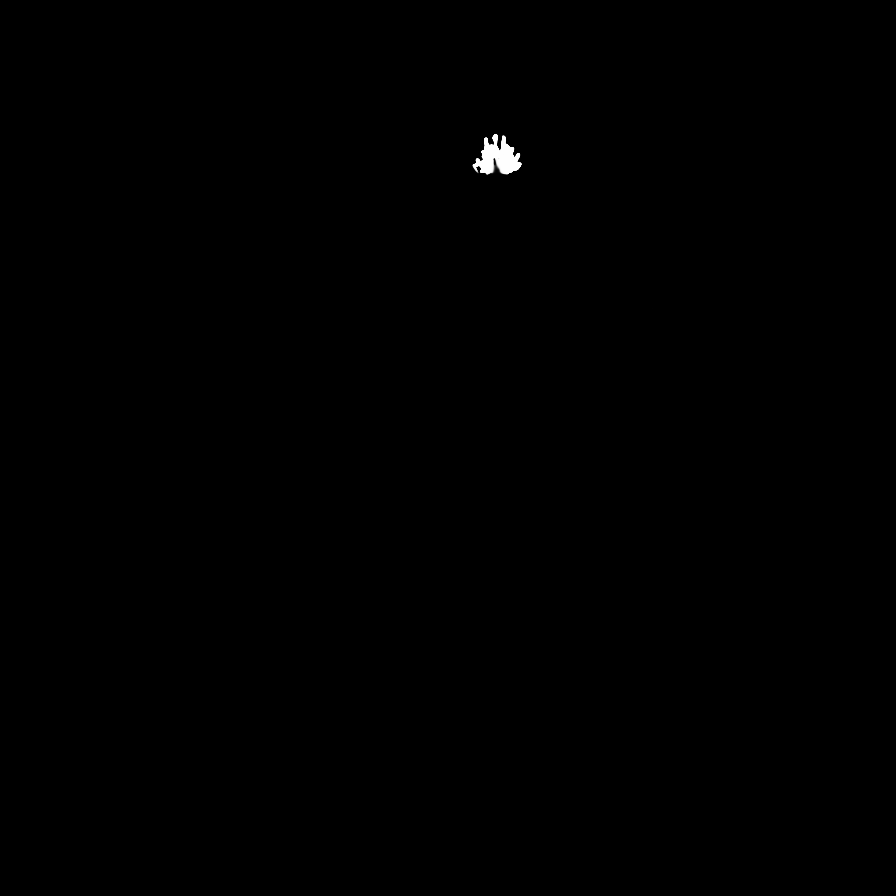
\includegraphics[width = 0.25\linewidth]{figures/000_flower.png}

    \vspace{1em}

    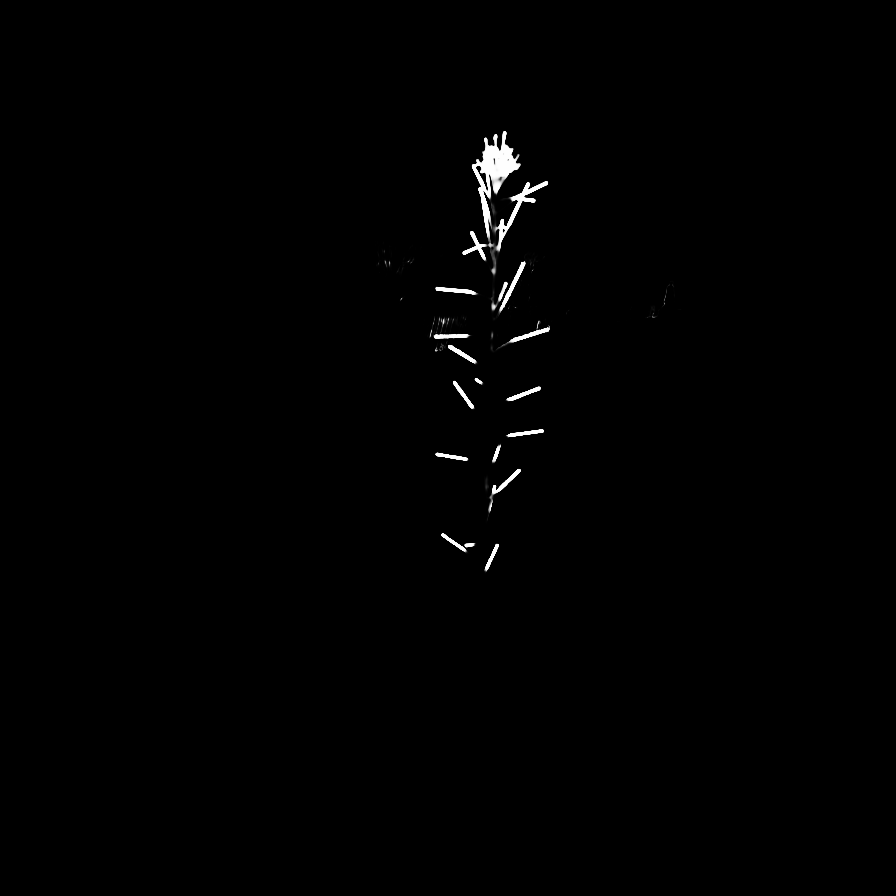
\includegraphics[width = 0.25\linewidth]{figures/000_fruit.png}\quad
    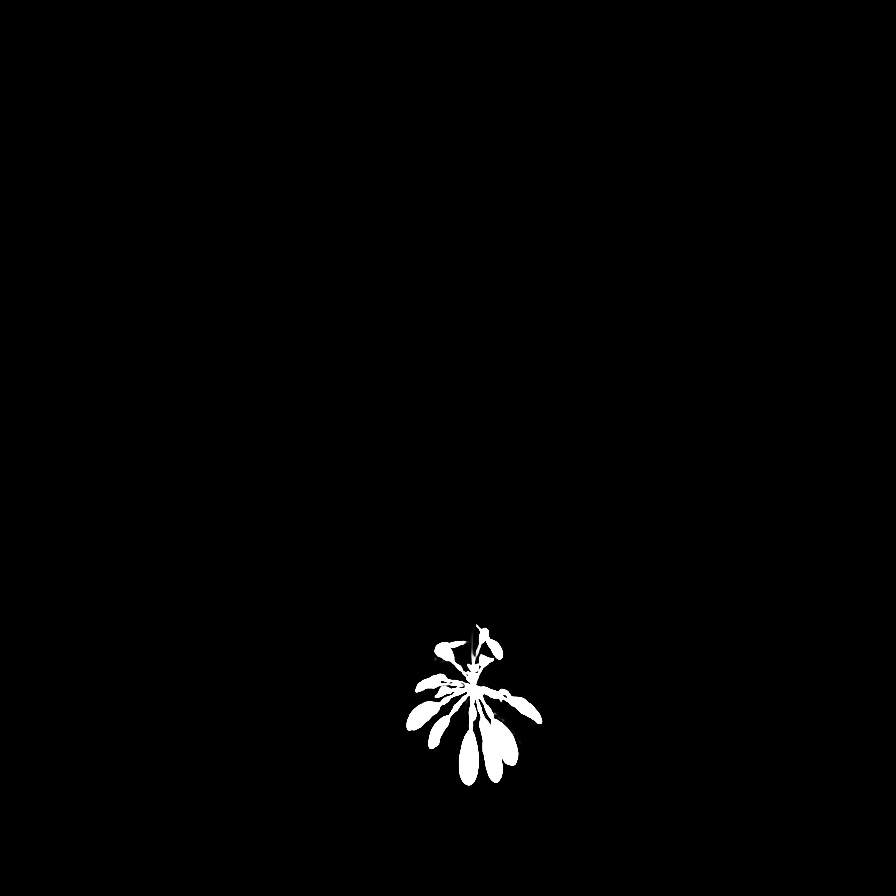
\includegraphics[width = 0.25\linewidth]{figures/000_leaf.png}\quad
    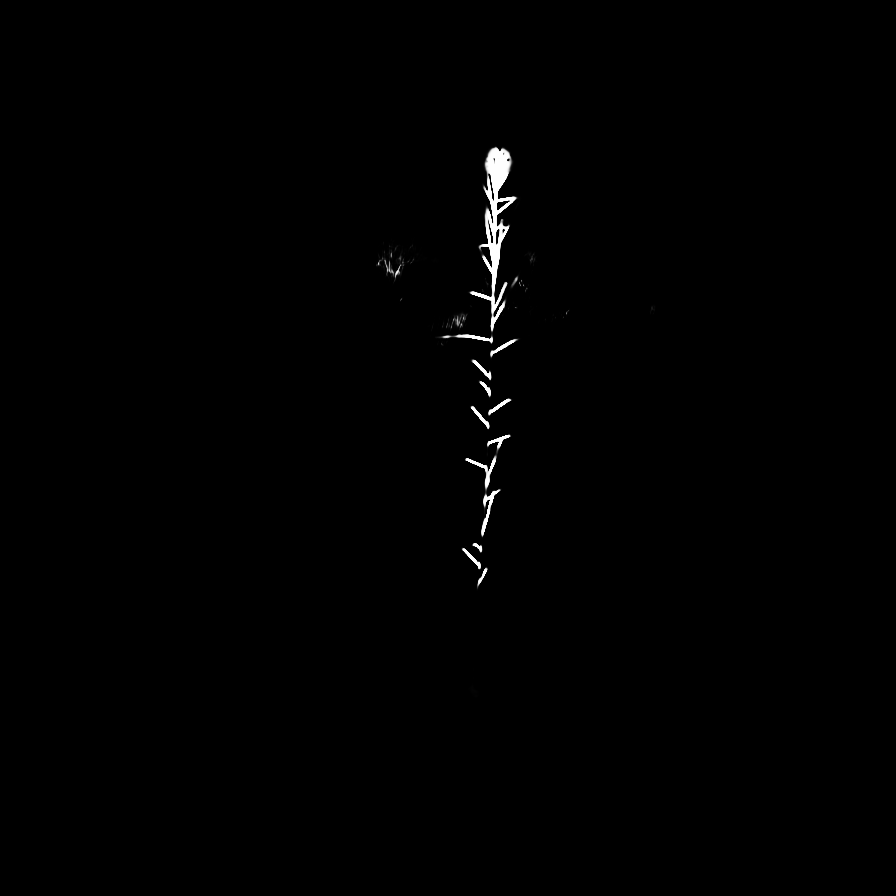
\includegraphics[width = 0.25\linewidth]{figures/000_pedicel.png}
    \caption{Images segmented with our network. From left to right, then top to bottom: original image,
        background, flower, fruit, leaf, pedicel. White indicates a high score (1.0) for the class,
        black indicates a low score (0.0).} \label{fig:seg2d_res}
\end{figure}

Pixels are classified using a threshold on the output of the segmentation
network: for each class $k$, if the score of a pixel is $>0.5$, then the pixel is
positively attributed to class $k$. Given the high contrast of the output images
from the neural netork, the chosen threshold does not matter much. Every pixel
$x$ in then attributed to one of four sets, as classical in the litterature:

\begin{itemize}
    \item $x$ belongs to $\textrm{TP}$ (true positive) if our predicted class is positive and the actual class is
positive;
    \item $x$ belongs to $\textrm{TN}$ (true negative) if our predicted class is negative and the actual class is
negative;
    \item $x$ belongs to $\textrm{FP}$ (false positive) if our predicted class is positive and the actual class is
negative;
    \item $x$ belongs to $\textrm{FN}$ (false negative) if our predicted class is negative and the actual class is
positive;
\end{itemize}

For voxels, the same classification is applied and each voxel is attributed a single class
from the segmentation algorithm presented above, and its class is compared to
the class of the closest point on the mesh produced by L-py.

For both pixels, and voxels, precision and recall are defined as follows and
used as a metric for the accuracy of segmentation:

$$
    \textrm{precision} = \frac{\textrm{\# TP} }{\textrm{\# TP} + \textrm{\# FP}},
    \textrm{recall} = \frac{\textrm{\# TP} }{\textrm{\# TP} + \textrm{\# FN}},
$$

Precision is the proportion of the predicted class which is correctly labeled,
recall is the proportion of all elements of a class which have been predicted.
Figure~\ref{fig:prec_recall_2d_3d} present precision and recall for each class
for both 2D and 3D segmentation. Voxels and pixels are accumulated over all of
dataset A. \\
\alien{The results show that the precision for each class is higher in 3D than in 2D. This is because the transfer to 3D reduces the number of false positives. Two reasons explainin the presence of false-positive in the 2D segmented images. First, the 3D reconstruction carves away the voxels based on the prediction of pixels onto they project. Therefore to avoid losing voxels that are part of the plant, we prefer  to favor false-positive against false-negatives on the 2D predictions and keep a low threshold to make the prediction masks. Second, the network is trained to predict overlaps of classes: one pixel can be attributed to multiple classes. This also favors false-positives over false-negatives. As stem, pedicel and fruits have similar structures (thin and elongated), the segmentation network tends to mix-up the classes and overlap predictions of these classes. However, when projecting in 3D only one class can be attributed per voxel. This class is the most probable class from all viewpoints, which allows to reduce the number of misattributions. On the other hand the first step of the 3D reconstruction consists in carving away all the voxels that are not belonging to the plant. If some pixels that were in the plant are removed in this step, it is impossible to recover them. Therefore the number of false negative increases in the 3D step, which has effect on the recall. This happens for the stem which is sometimes discontinuously reconstructed due to error of prediction on the background class. The false negatives also come from misattribution of class. For example the flowers are very thin, small and surrounded by other organs which makes them hard to predict precisely. It is also significant at organ intersections, for example where the pedicel are branched to the stem. }{These results show that precision is roughly equal or slightly better
for almost all classes in 3D than in 2D, but recall suffers on classes which are
occluded a lot: some parts of the stem and some flowers on the top of the plant
models are occluded by pedicel and fruits on almost all pictures, which explains
why some part of it are missed.}


\begin{figure}[h!]
    \centering 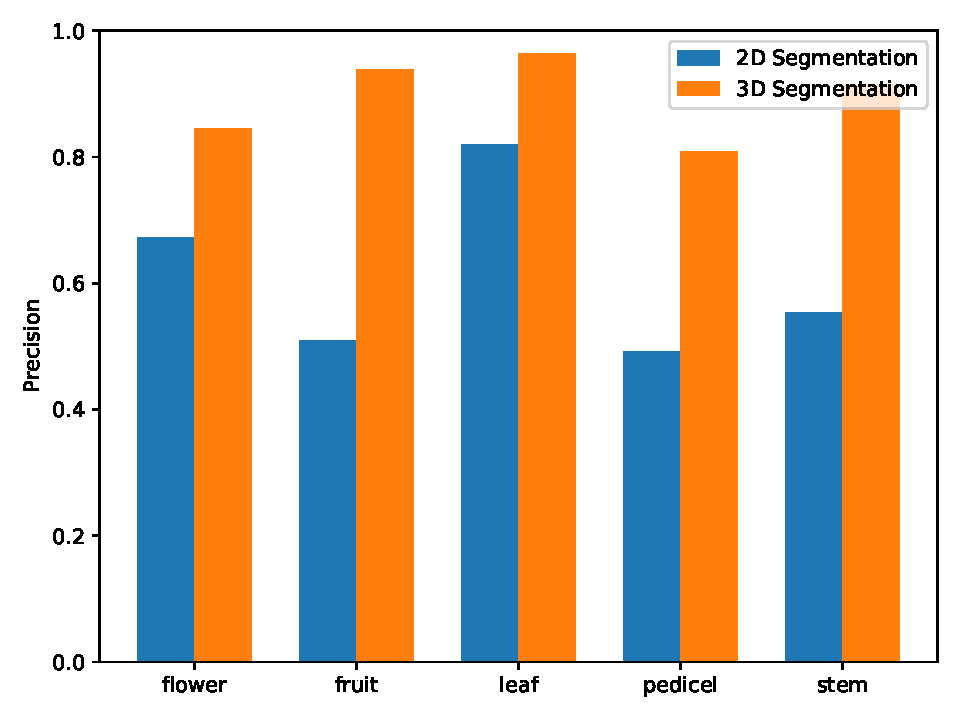
\includegraphics[width = 0.5\linewidth]{figures/eval_precision.pdf}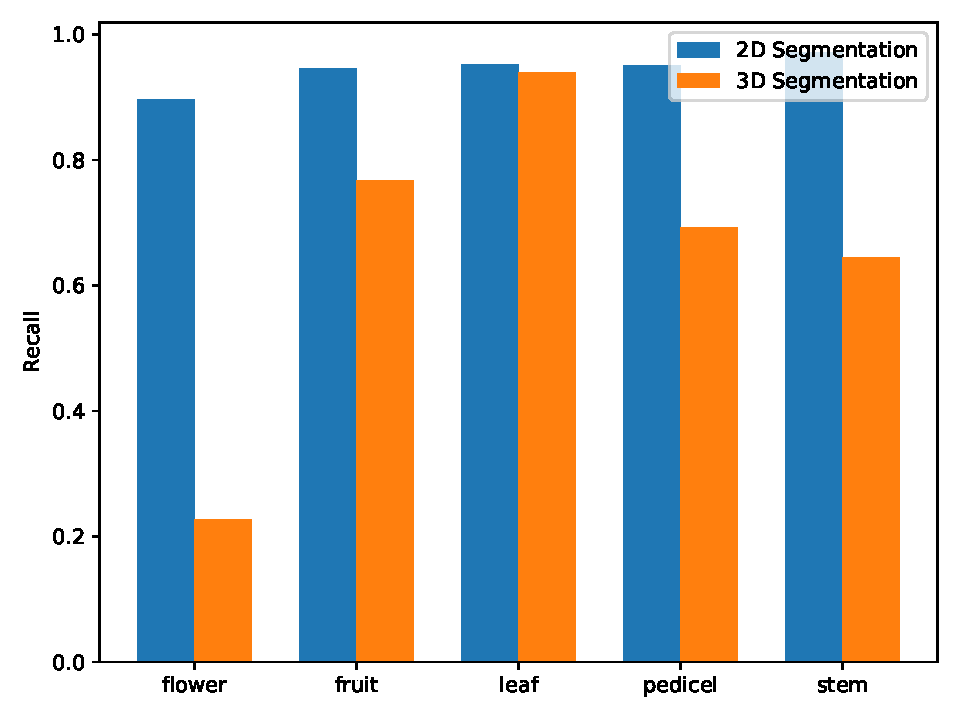
\includegraphics[width = 0.5\linewidth]{figures/eval_recall.pdf}
    \caption{Precision and recall comparison between 2D segmentation and 3D
segmentation.} \label{fig:prec_recall_2d_3d}
\end{figure}


\paragraph{2D Segmentation of real arabidopsis.}
 We then manually annotated real images of \emph{A. Thaliana} (dataset B) and evaluated the performance of the model trained on the virtual dataset. We present precision and recall results for each class, comparing results on virtual plants and real plants (Figure \ref{fig:prec_recall_virt_real}). It has to be noted that the size of the dataset (6 pictures) is small and limiting for proper statistical analysis. Although the network makes more errors than with the virtual plants, we get satisfactory segmentation results. Among the errors, mix-up between the stem, fruit and pedicel classes is more present and the network has difficulties distinguishing fruits and leaves when they grow along the setm. Observing the errors made by the network allowed us to improve the 3D models of the plants based on the errors the segmentation was making: we included rotation of the leaves, bending of the stem and random coloration of the organs. This allowed to both improve the plant models and the 2D-segmentation network. Overall, the 3D models of the plant and the images generated in the virtual environment are good enough to obtain a satisfactory segmentation of the plants and especially on the 3D reconstruction of the real plants.\\


\begin{figure}[h!]
    \centering 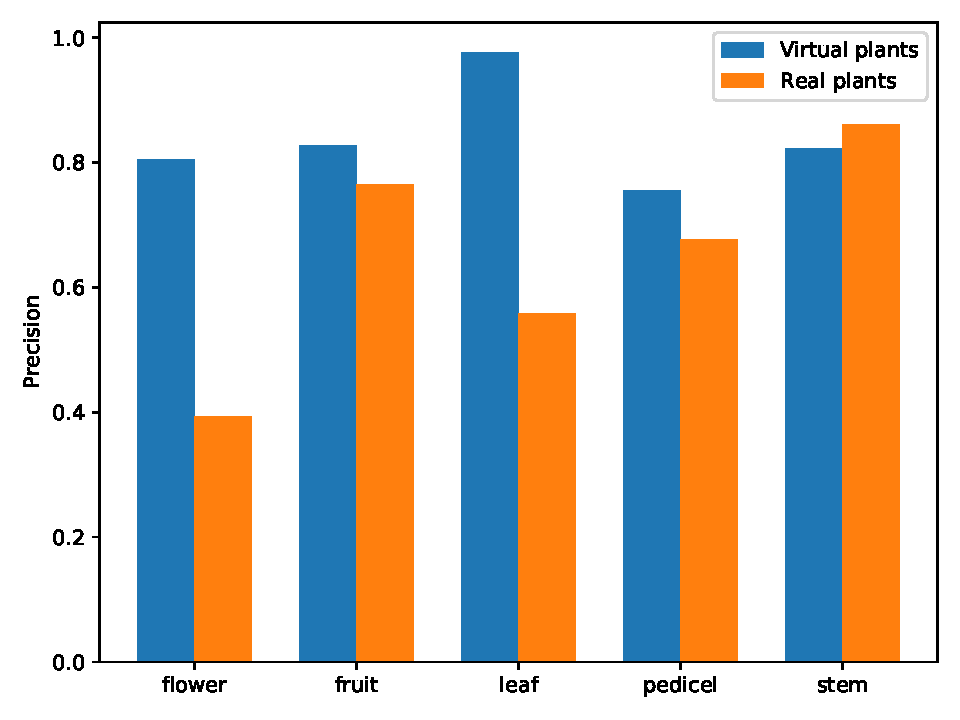
\includegraphics[width =
0.5\linewidth]{figures/eval_precision_real.pdf}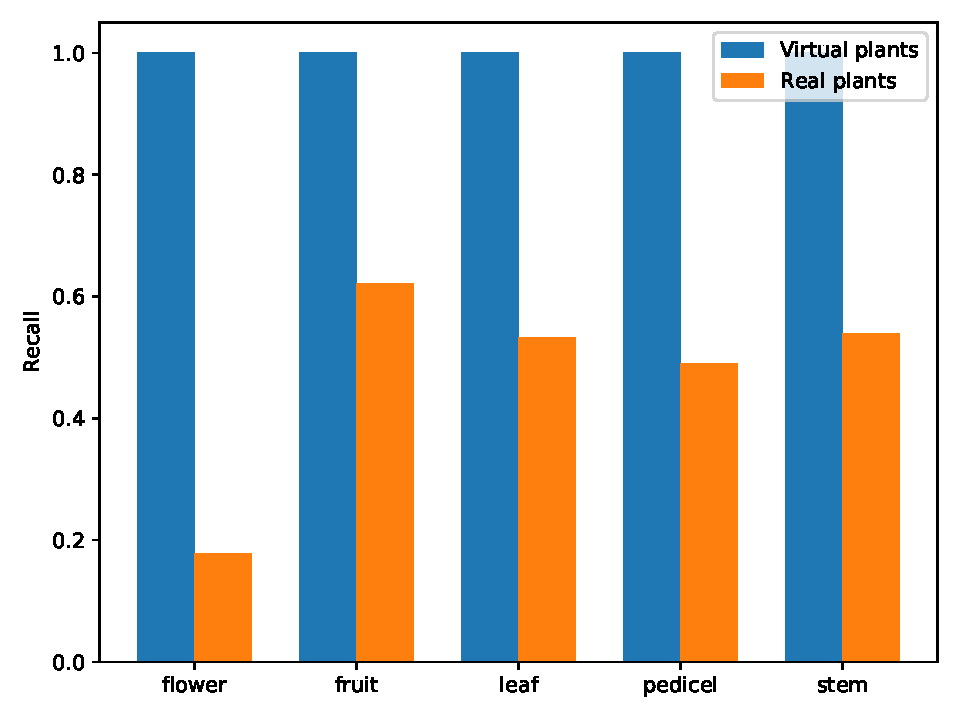
\includegraphics[width =
0.5\linewidth]{figures/eval_recall_real.pdf}
    \caption{Precision and recall comparison between 2D segmentation on
virtual and real images unseen by the neural network.} \label{fig:prec_recall_virt_real}
\end{figure}

\paragraph{Qualitative evaluation on real plants.}
We then segmented and reconstructed  \emph{A. Thaliana} real plants from dataset C. Some example pictures are shown on Figure \ref{fig:realscans}. Without ground truths we can only give a qualitative analysis of the results (Figure \ref{fig:rec3d}). The reconstructions and segmentation were qualitatively as good as the 3D reconstruction to the point where in some cases it is hard to tell whether the reconstructed plant is from a real or a virtual plant. One default is that the reconstruction of the leaves at the basis on the stem is not accurate. This is due to the fact that these leaves are hardly identifiable, mixed with the pot or dried out. They are of little phenotypical interest so we didn't focus on solving this issue. Another issue comes from occlusions, especially of the stem. The reconstruction fails for example when there are several plants grouped together in ths same pot, or when there is a structure unknown to the segmentation network, for example a tutor obstructing some viewpoints. To solve the first issue one solution would be to increase the variety in the viewpoints, by taking pictures from the top of the pot. To solve the second, we would need to teach the network to interpret occlusions by foreign objects, by including such objects in the virtual scene for example.

\begin{figure}[h!]
    \centering 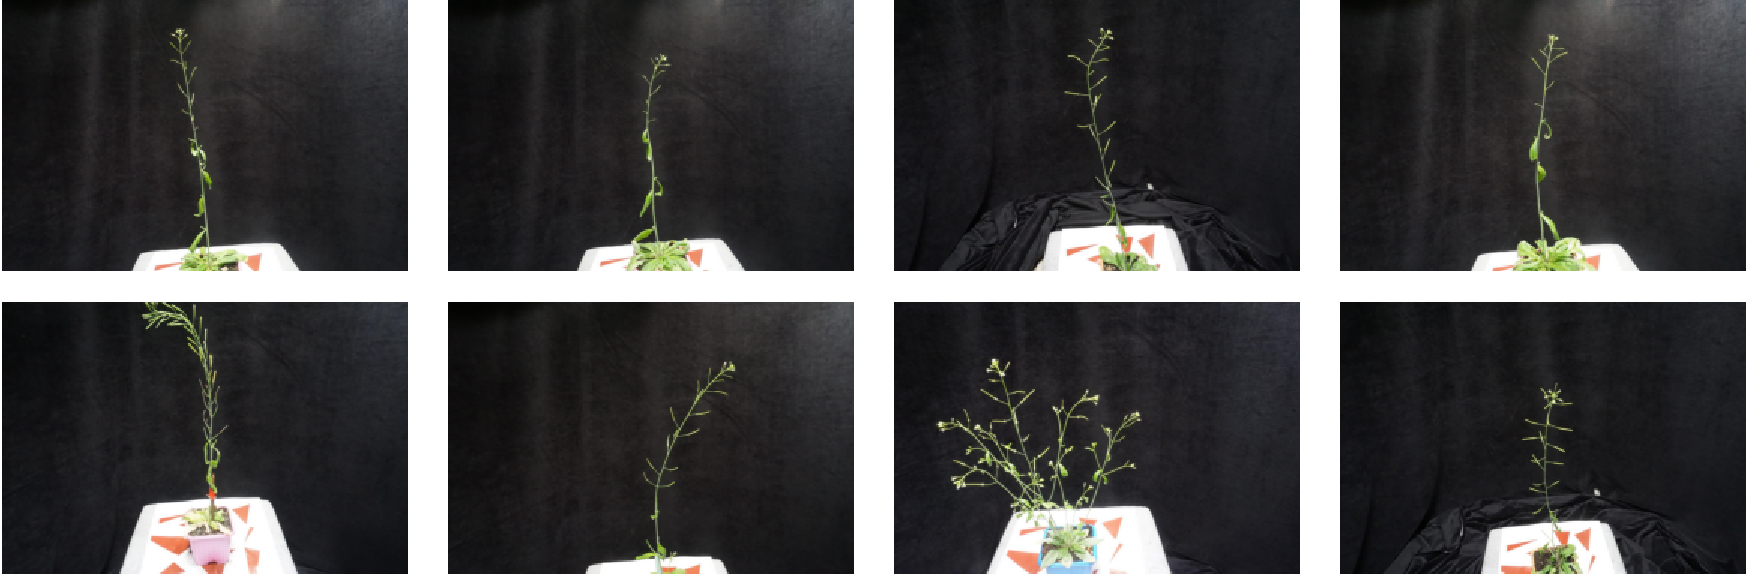
\includegraphics[width = \linewidth]{figures/seg-crop.pdf}
    \caption{Sample images from the dataset used for qualitative assessment of the method on real data} \label{fig:realscans}
\end{figure}

\begin{figure}[h!]
    \centering 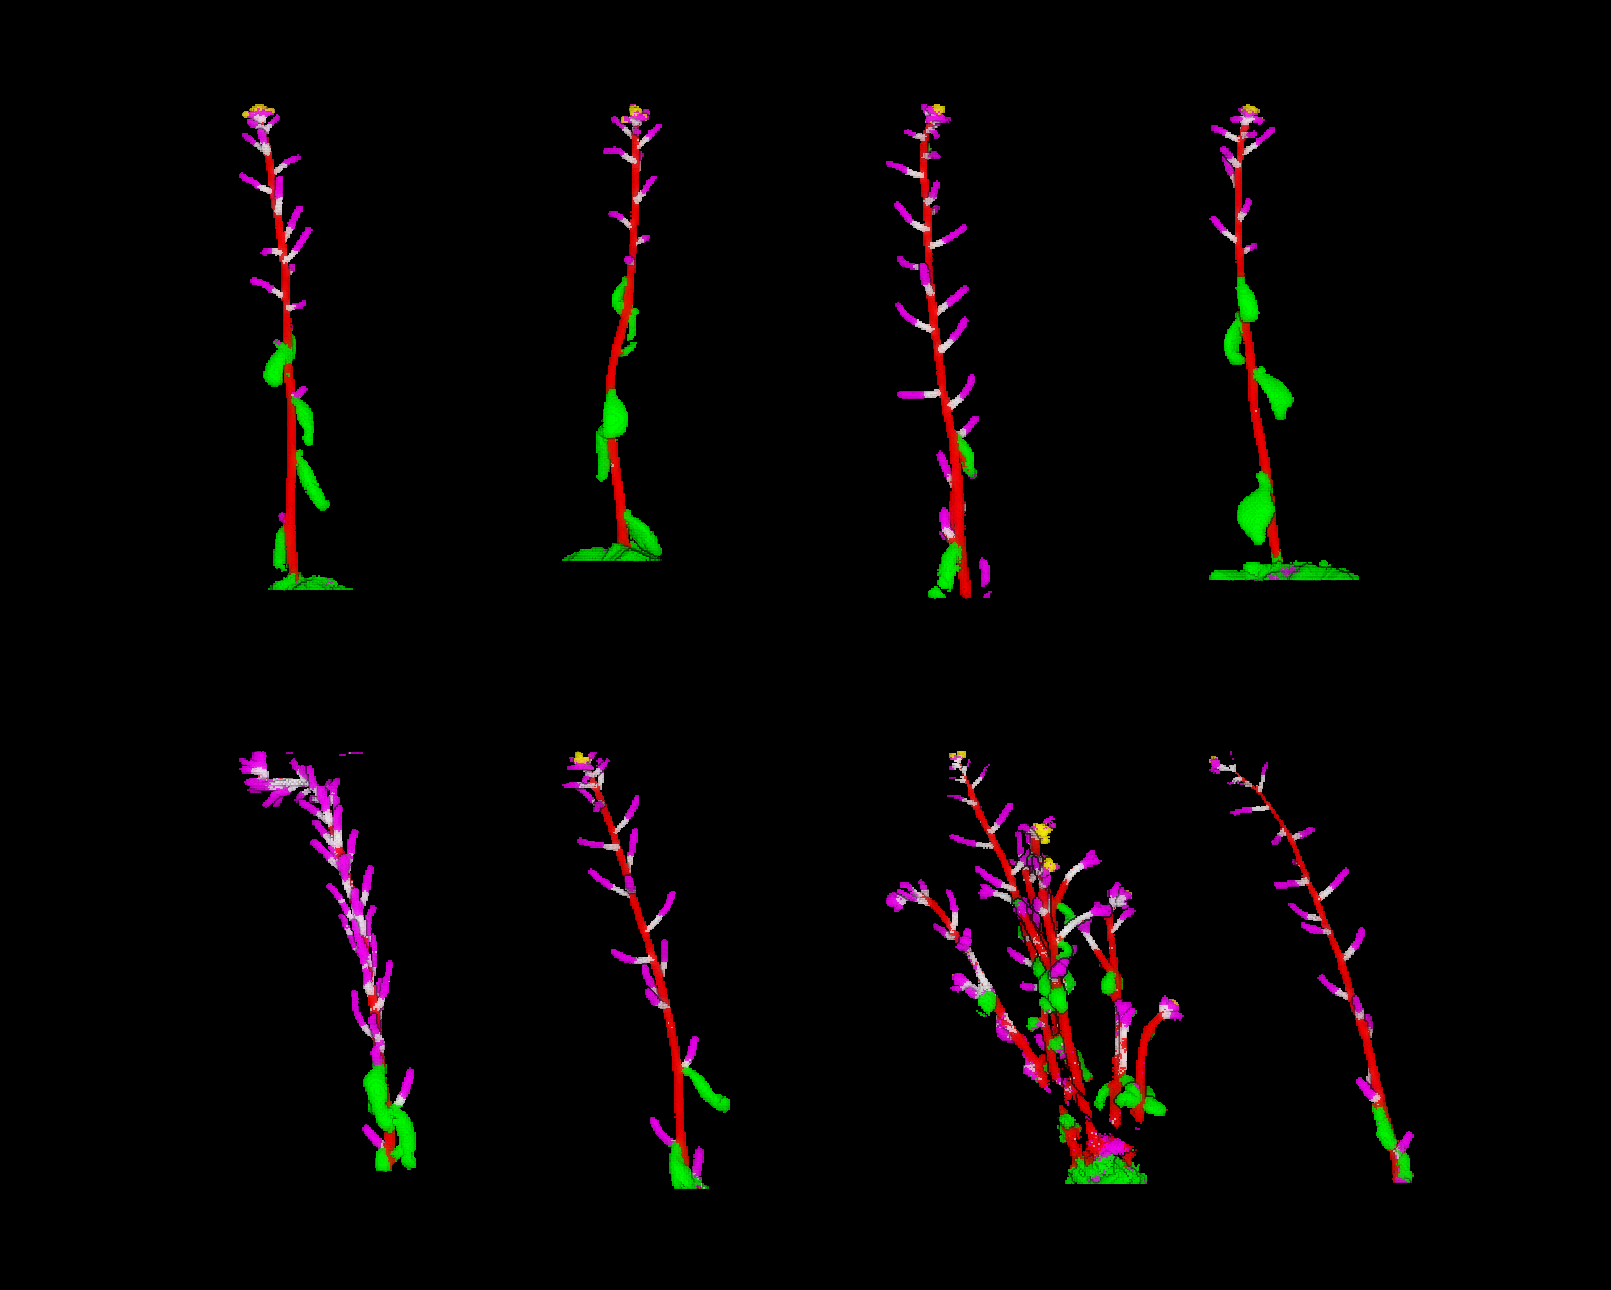
\includegraphics[width = 0.7\linewidth]{figures/capture.png}
    \caption{3D reconstruction of real plants. Red: stem, green: leaf, white: pedicel, purple: fruit:, yellow: flower} \label{fig:rec3d}
\end{figure}

\paragraph{Transfer to other species.}
To transfer to species anatomically different from \emph{A. Thaliana} we used model finetuning. This step requires a minimal number of manually annotated images (2 or 3) of the other species and allows to reconstruct the full model in 3D. To test the finetuning method we took a video turning around a tomato plant and sampled 41 images equally distributed along the video to get images from different viewpoints. Then 2 images were manually annotated with our interface. We included only the two classes present: stem and leaf. Then the network trainied on virtual \emph{A. Thaliana} was trained on these two images for 20 epochs. Then we ran the 2D segmentation (Figure \ref{fig:finetune2D}) 3D reconstruction pipeline and obtained a 3D model of the tomato (Figure \ref{fig:finetune3D}). We notice that the reconstruction of the plant at the level encompassed properly in the field of view of the camera is correct. However the top leaves reconstruction suffers from lack of information. To improve the quality of the reconstruction more points of view of the tomatoe would have been needed. 

\begin{figure}[h!]
    \centering 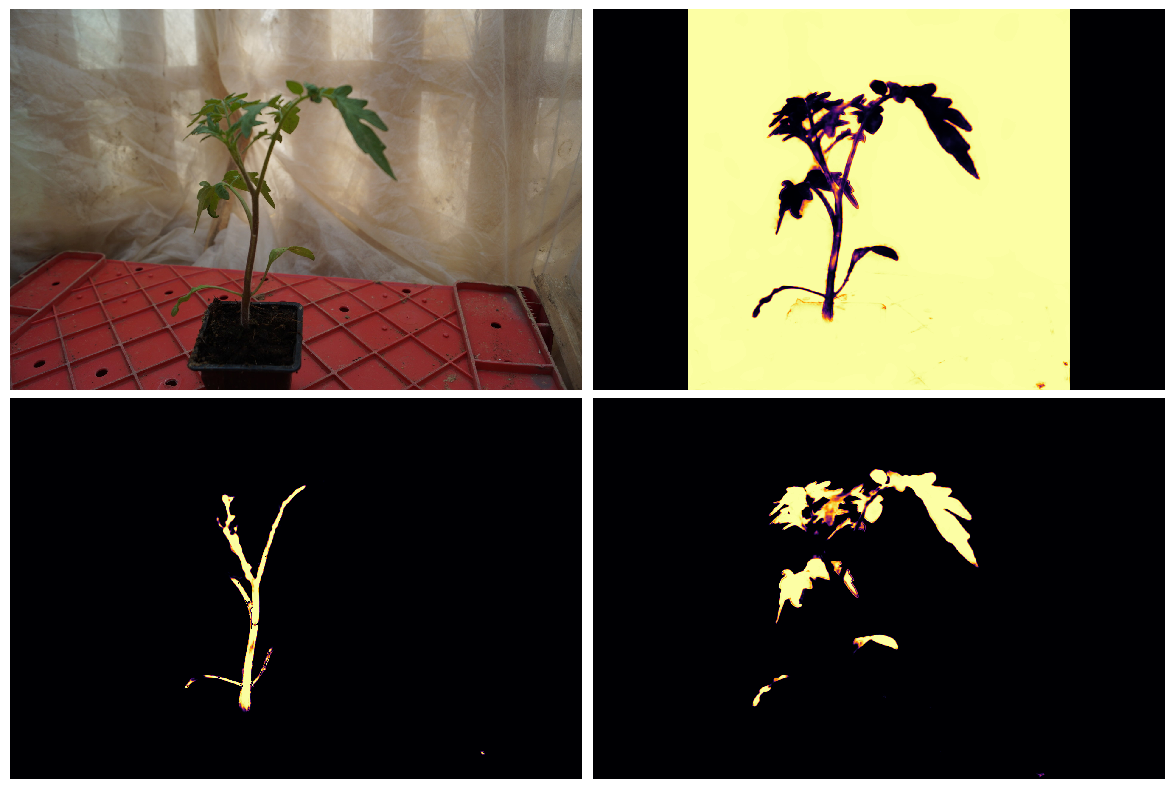
\includegraphics[width = \linewidth]{figures/finetune.png}
    \caption{Predictions of the model finetuned on two images of tomato manually annotated. (The masks of pedicel and stem are superimposed on this figure but they were predicted separately).} \label{fig:finetune2D}
\end{figure}


\begin{figure}[h!]
    \centering 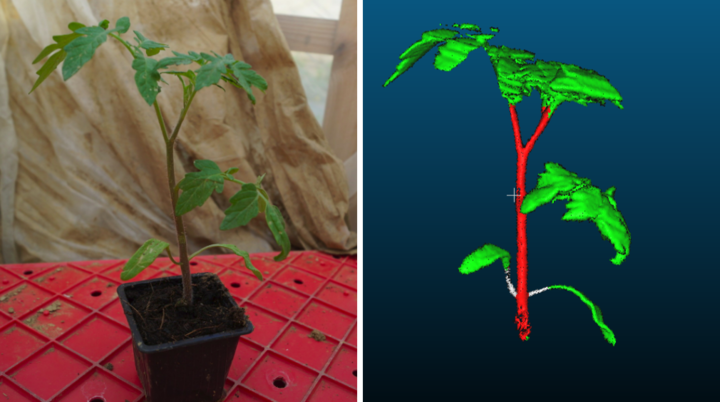
\includegraphics[width = \linewidth]{figures/tomato.png}
    \caption{3D reconstruction and segmentation of tomato plant with the pipeline.} \label{fig:finetune3D}
\end{figure}





\section{Conclusion and perspectives}
In this work, we have presented and assessed a fullly automated method for segmentation of
plants from 2d pictures using convolutional networks for segmentation in 2d and
backprojection of 3d points for segmentation in 3d.

The most noteworthy conclusion from this work is that we have demonstrated that using generative
models of plants for training neural networks and apply the trained algorithms
on real specimen of plants is robust enough that no additional annotation of
data is needed. This is of utmost importance to the field of plant biology, since annotation of data
is very time-consuming, and the variety in plant species makes
the never-ending annotation of new species a never ending task.

We have also shown that minimal annotation of real world data can be enough to
transfer the models to very different plants. These tests done on small datasets
only call for further investigation of how well the models can generalize to whole
classes of plants when mixing several plant models together. We are confident
that they indeed generalize well, given the recent successes in using
convolutional neural network for segmentation tasks, but it would need to
develop or adapt generative models of other plant species.

Another perspective of work is to investigate whether the obtained segmentation is precise
enough that we can use it to gather quantitative data on the plant themselves,
as this would prove to be very valuable to many fields in plant biology. A
testing procedure will be developped and compared to more traditional geometry
based approaches for the specific application of measuring the phyllotactic
angles of Arabidopsis thaliana.


{\small
\bibliographystyle{ieee_fullname}
\bibliography{biblio.bib}
}

\end{document}
